\section{Background}
\label{sec:Background}
In this section, we formally describe the definitions of KPI firstly (Section~\ref{subsec:kpi}). Secondly, we introduce the core idea of general PU learning (Section~\ref{subsec:PU learning based methods})  as well as active learning (Section~\ref{subsec:Active Learning}) and their application in our scenario. Lastly, we introduce the clustering methods of KPI streams (Section~\ref{subsec:clustering}).

\begin{figure*}
    \centering
	  \subfloat[step1]{
	  \begin{minipage}[t]{0.45\linewidth}
      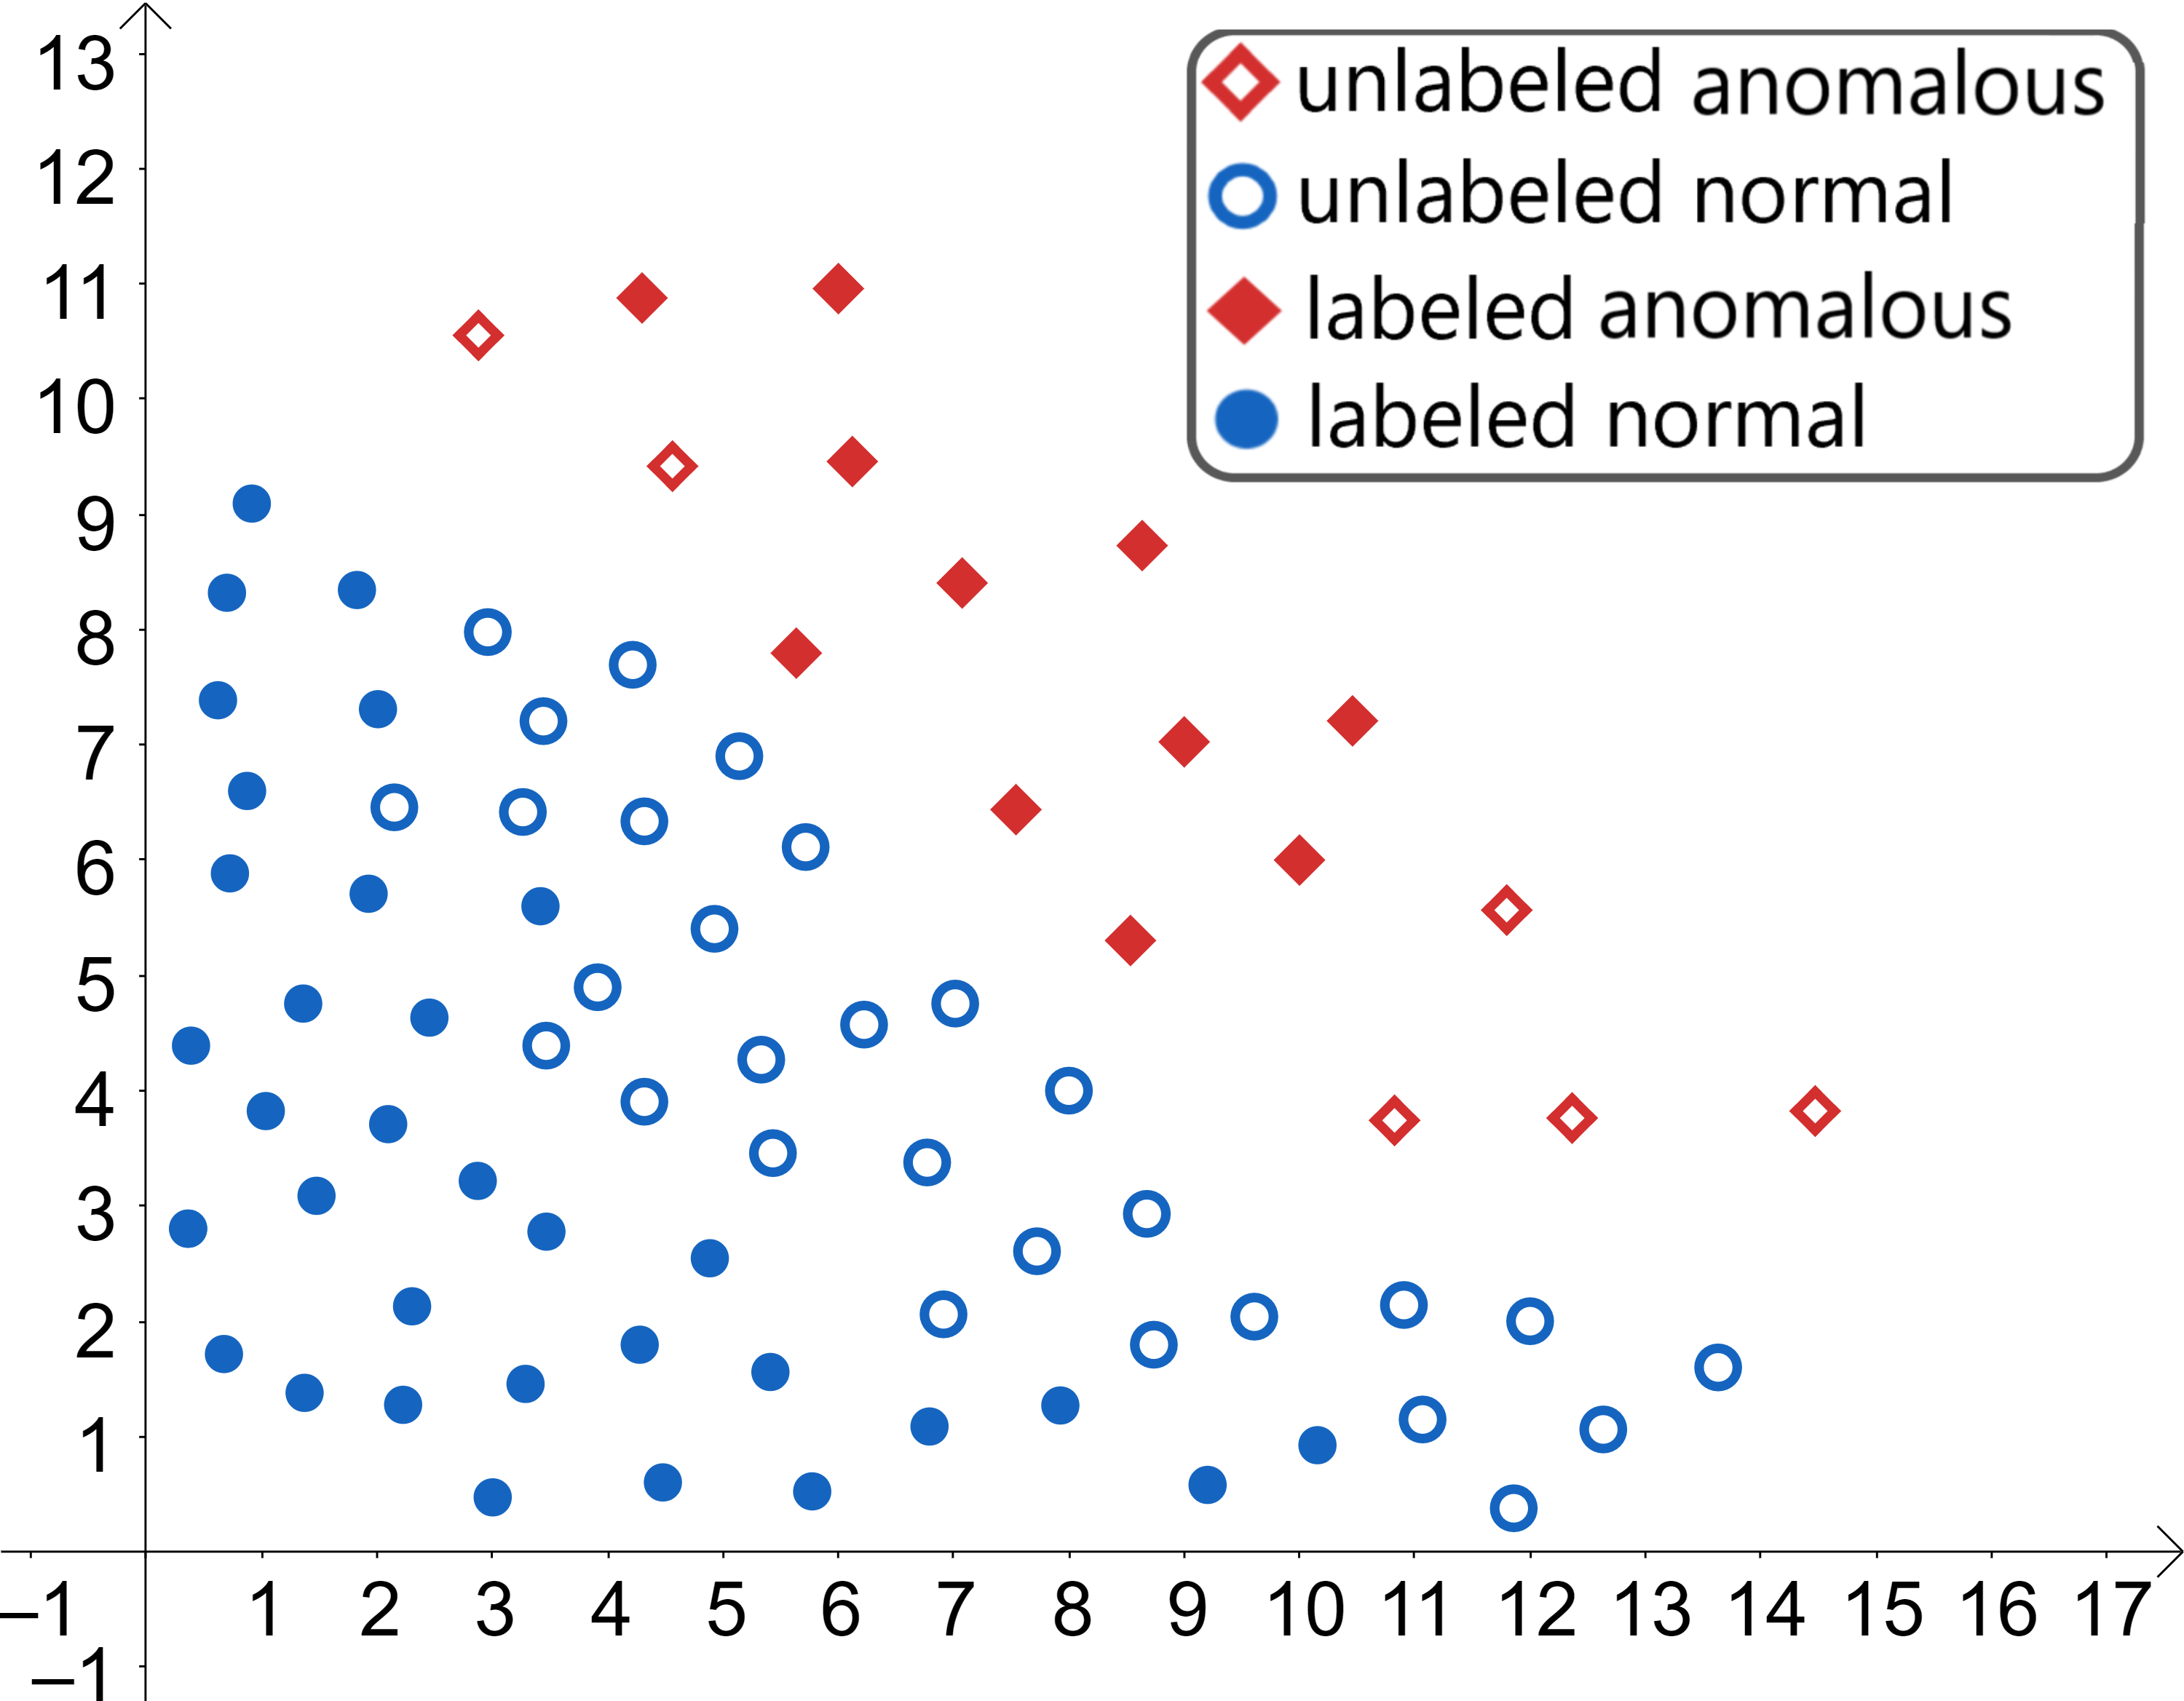
\includegraphics[width=2.6in]{ADS_Journal/PU figures/step1.png}\label{1a}
      \end{minipage}}
	  \subfloat[step2]{
	  \begin{minipage}[t]{0.45\linewidth}
      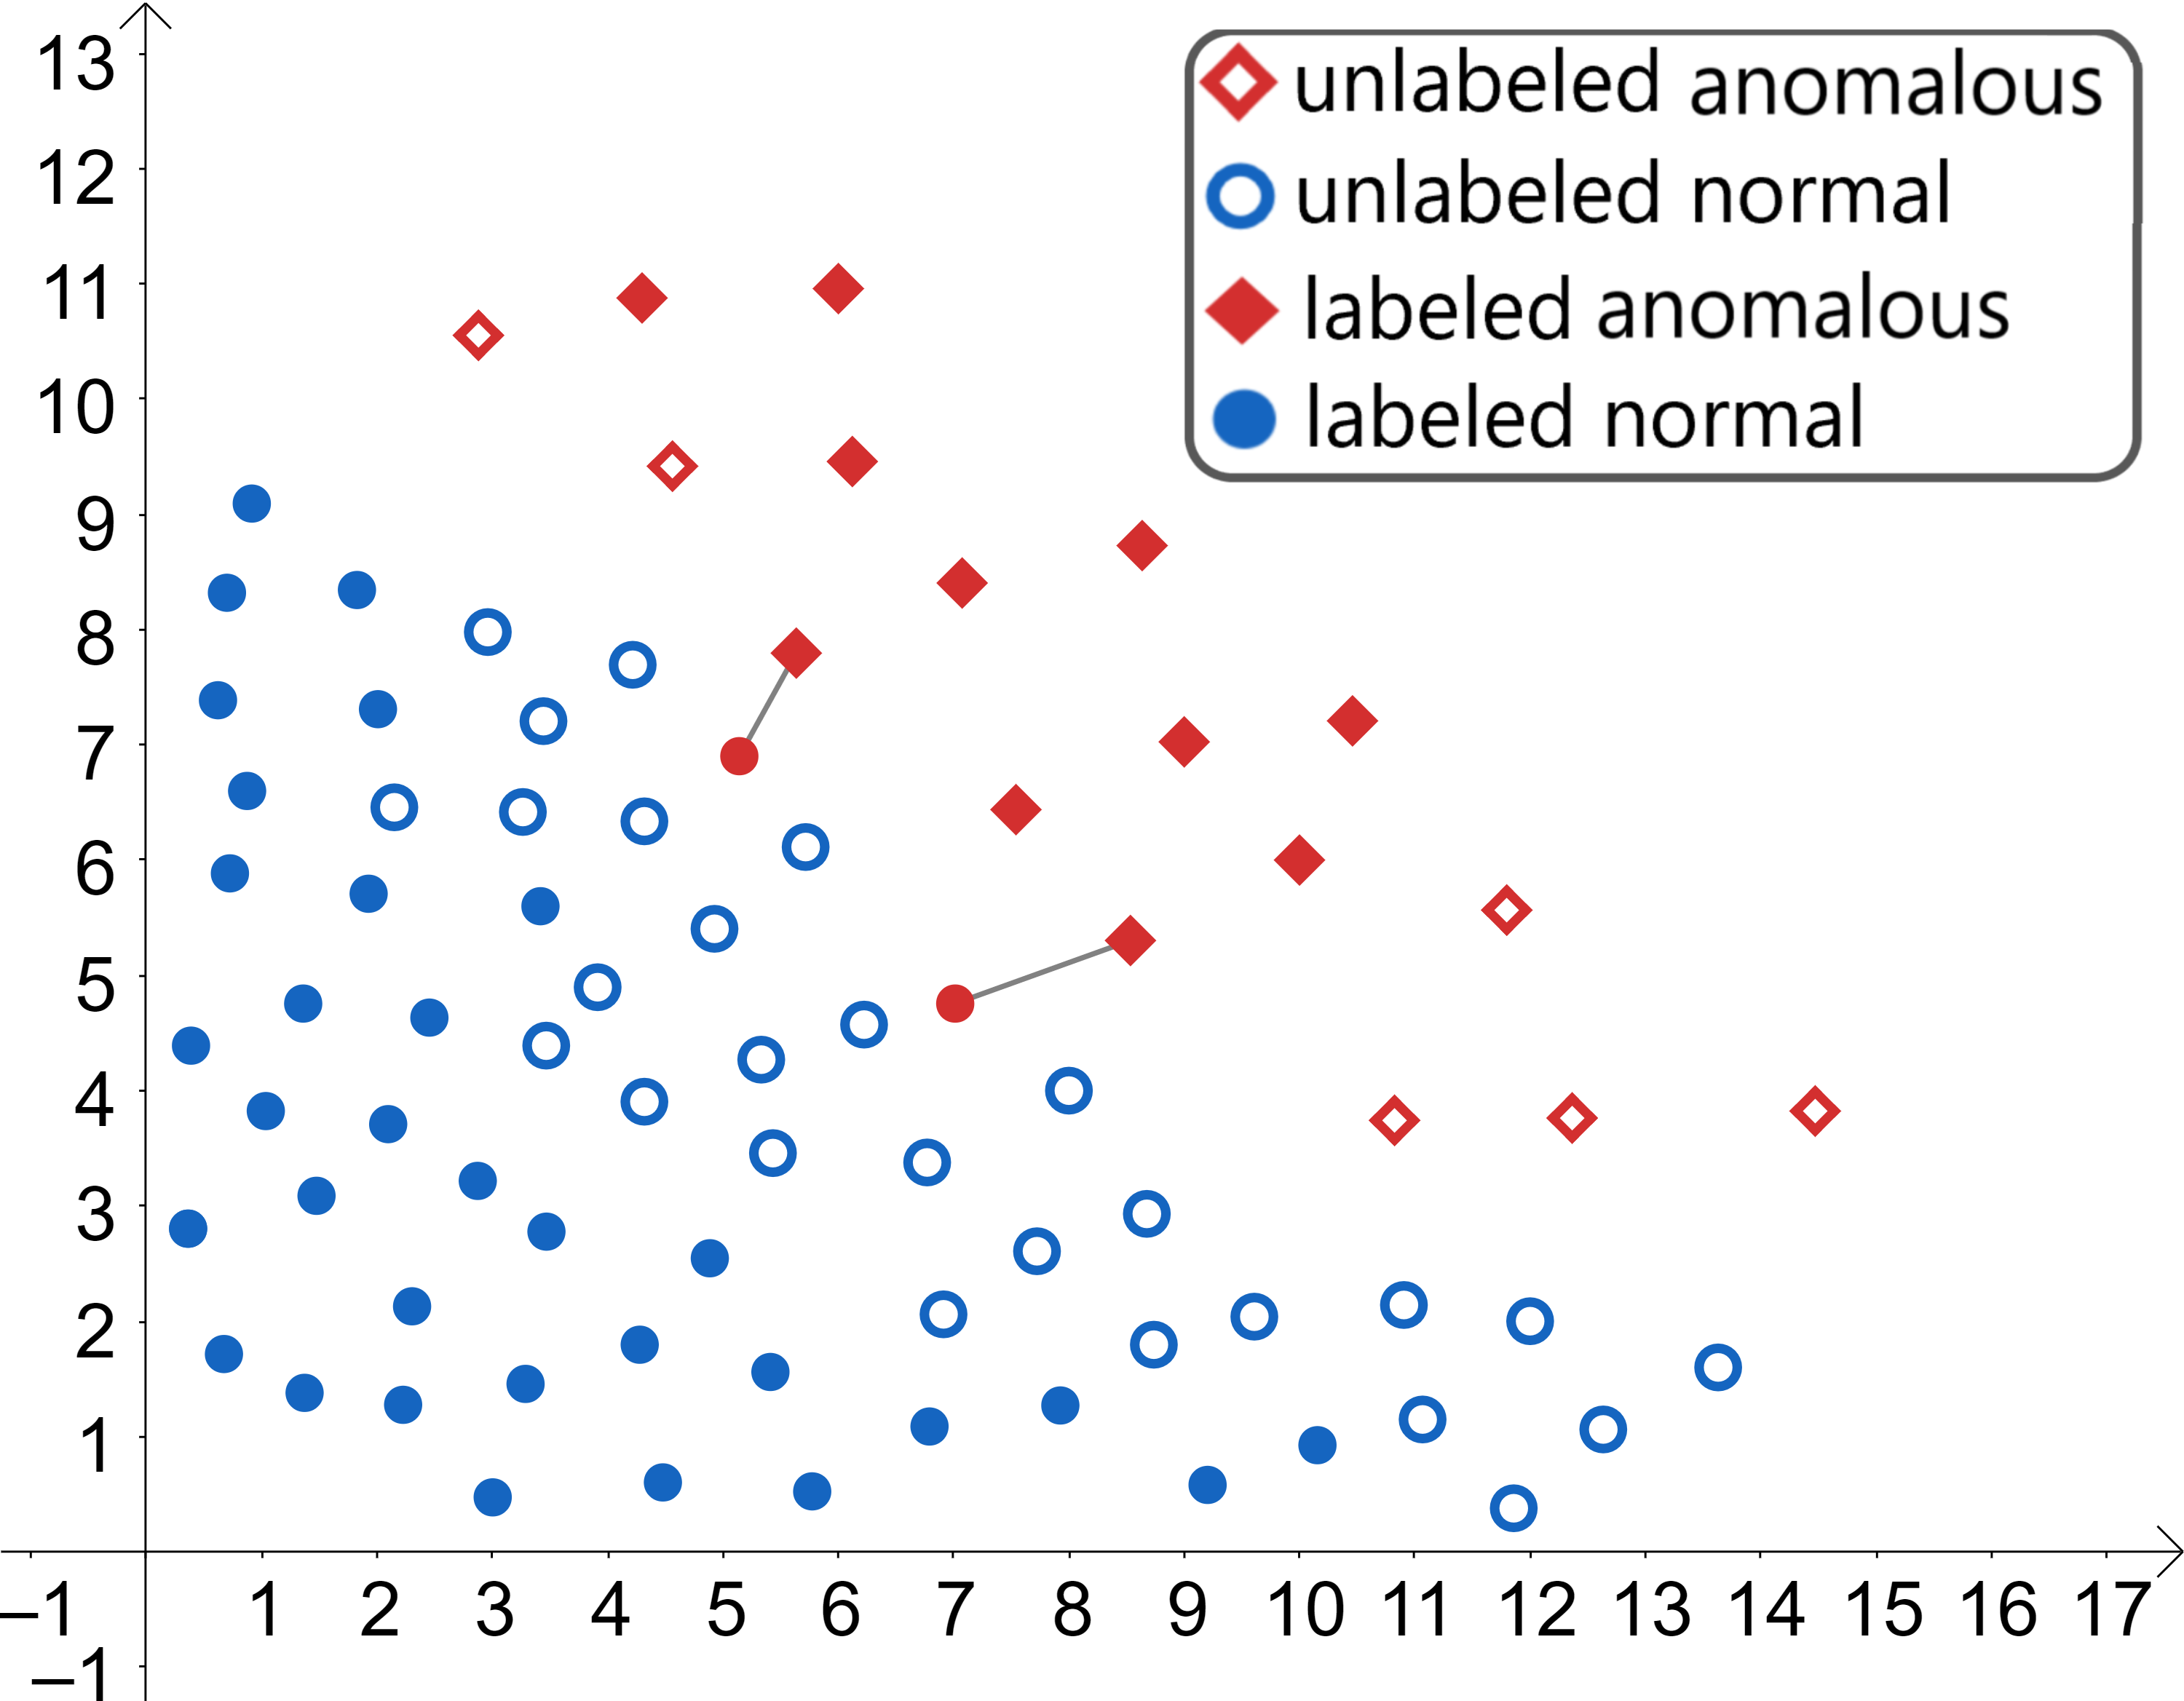
\includegraphics[width=2.6in]{ADS_Journal/PU figures/step2.png}\label{1b}
      \end{minipage}}
      
      \vspace{0.3in}
	  \subfloat[step3]{
	  \begin{minipage}[t]{0.45\linewidth}
      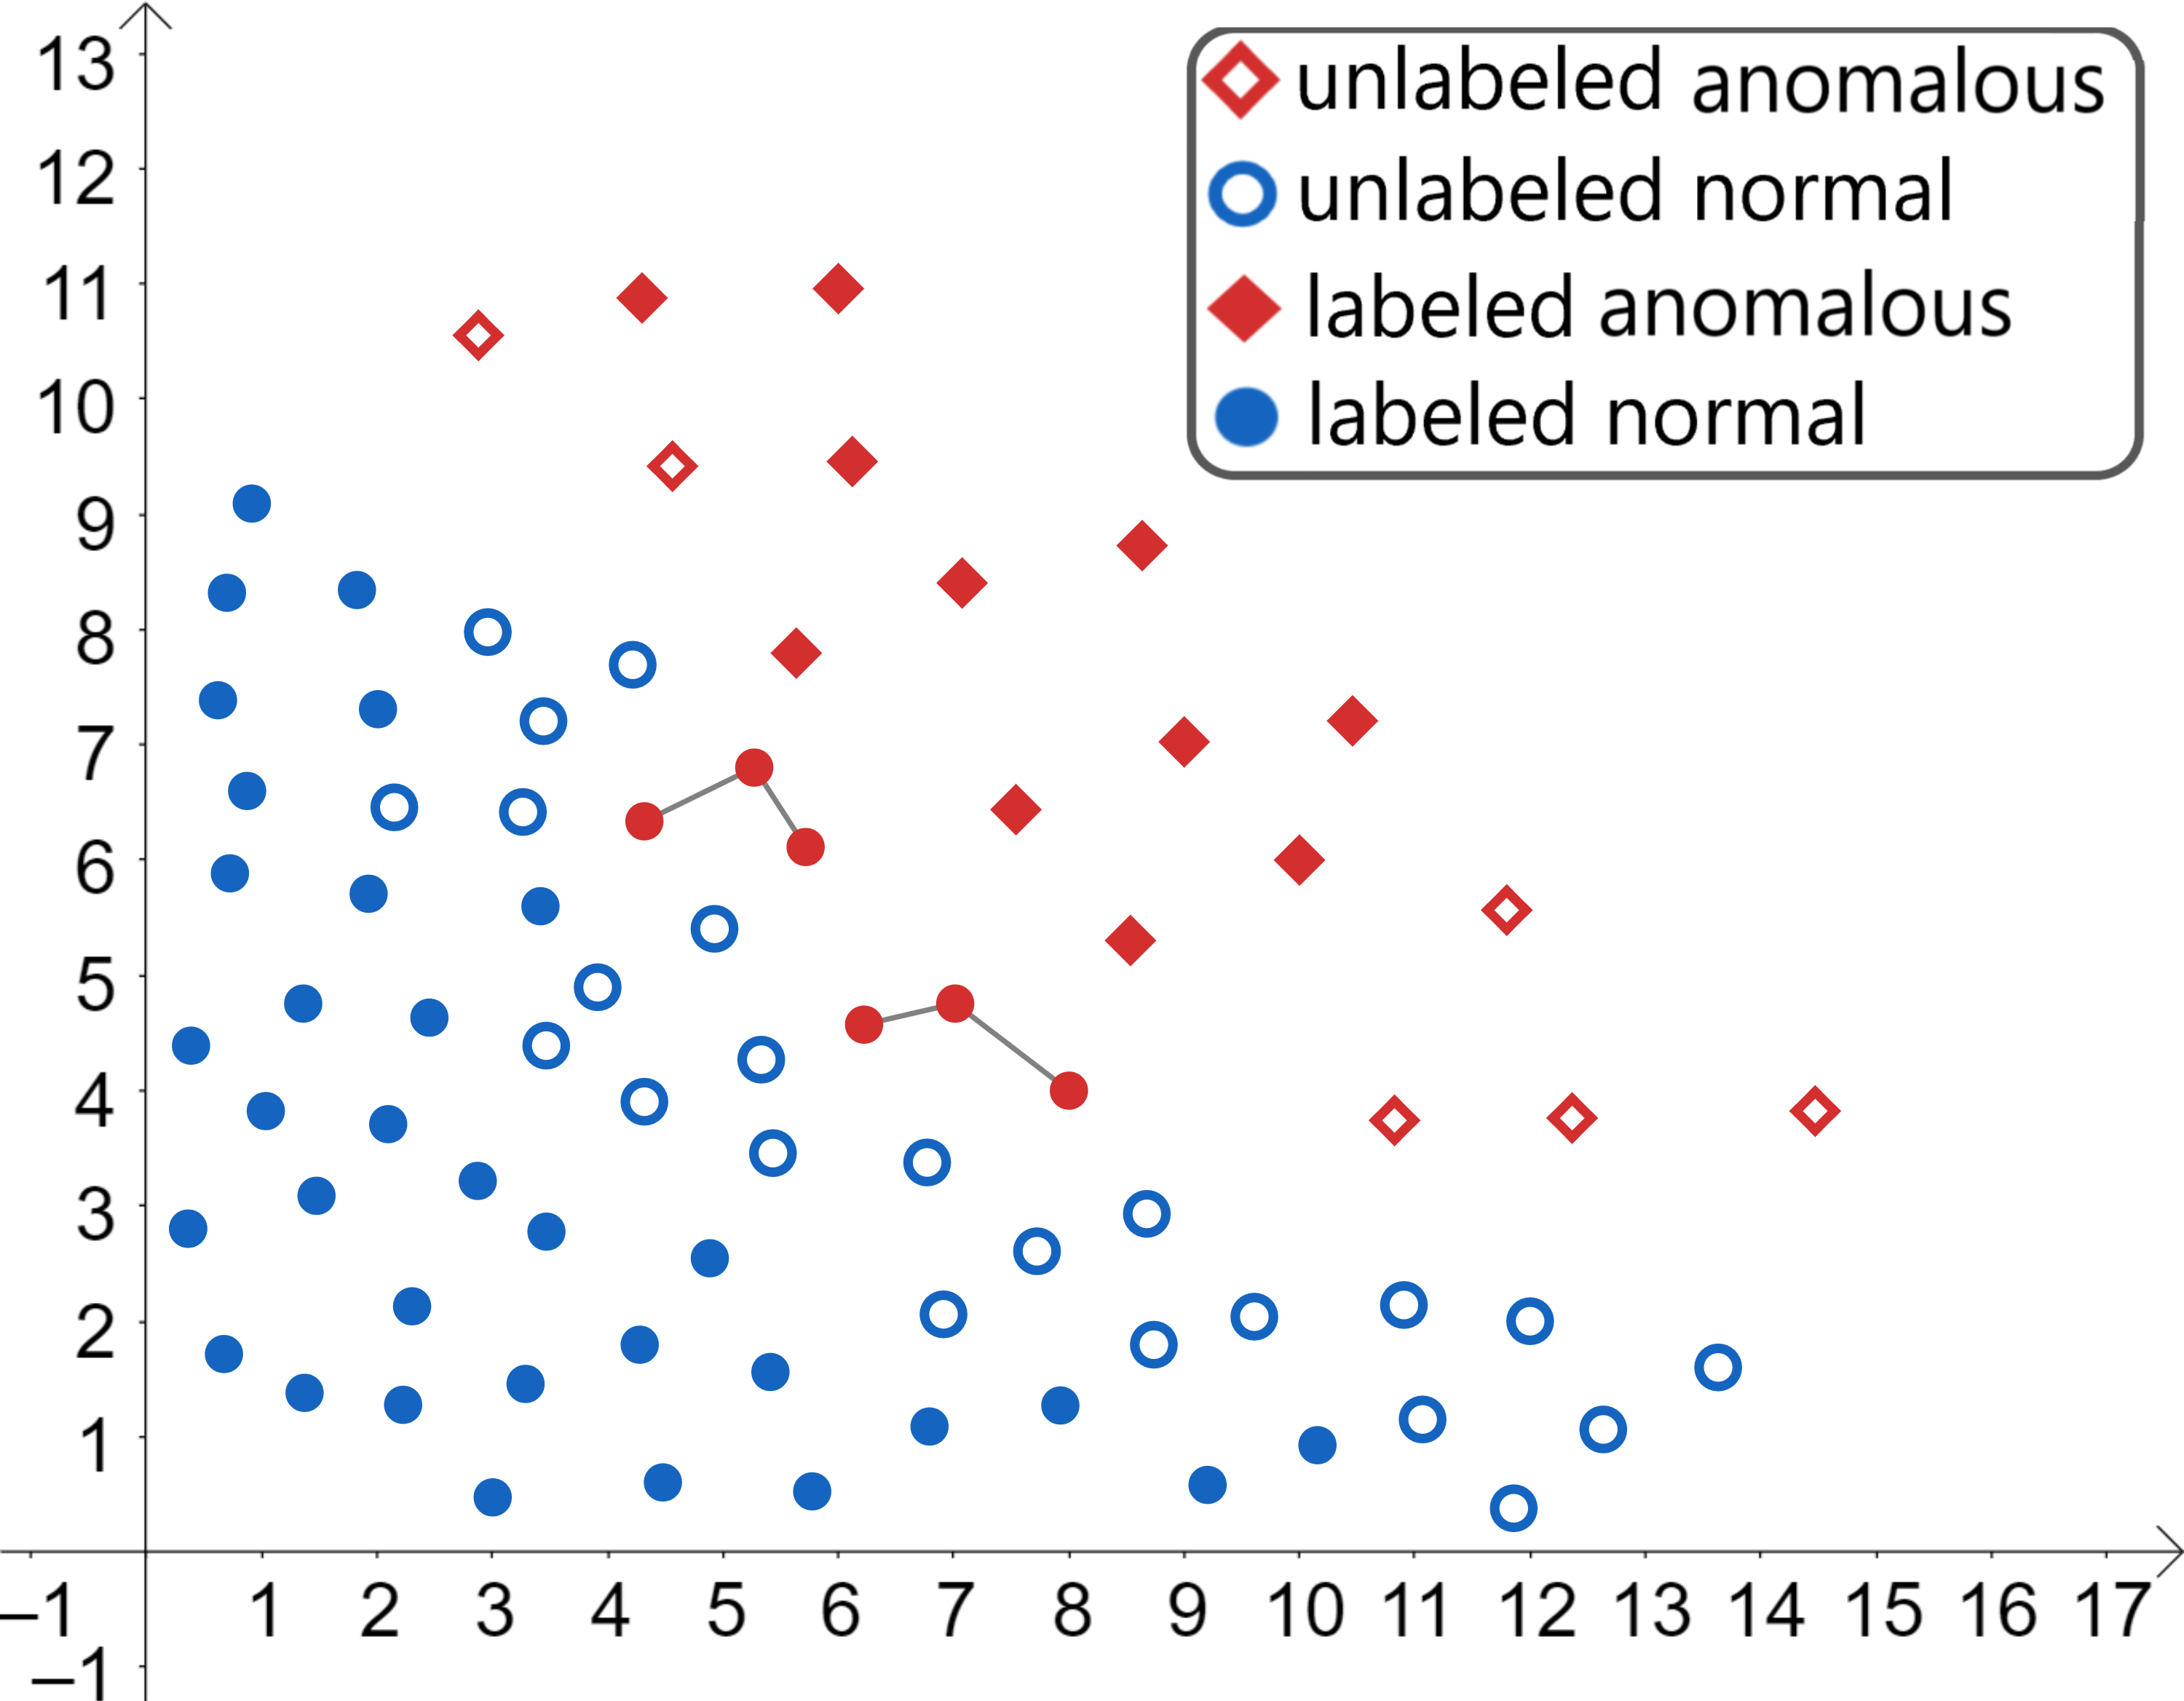
\includegraphics[width=2.6in]{ADS_Journal/PU figures/step3.png}\label{1c}
      \hfill
      \end{minipage}}
	  \subfloat[step4]{
	  \begin{minipage}[t]{0.45\linewidth}
      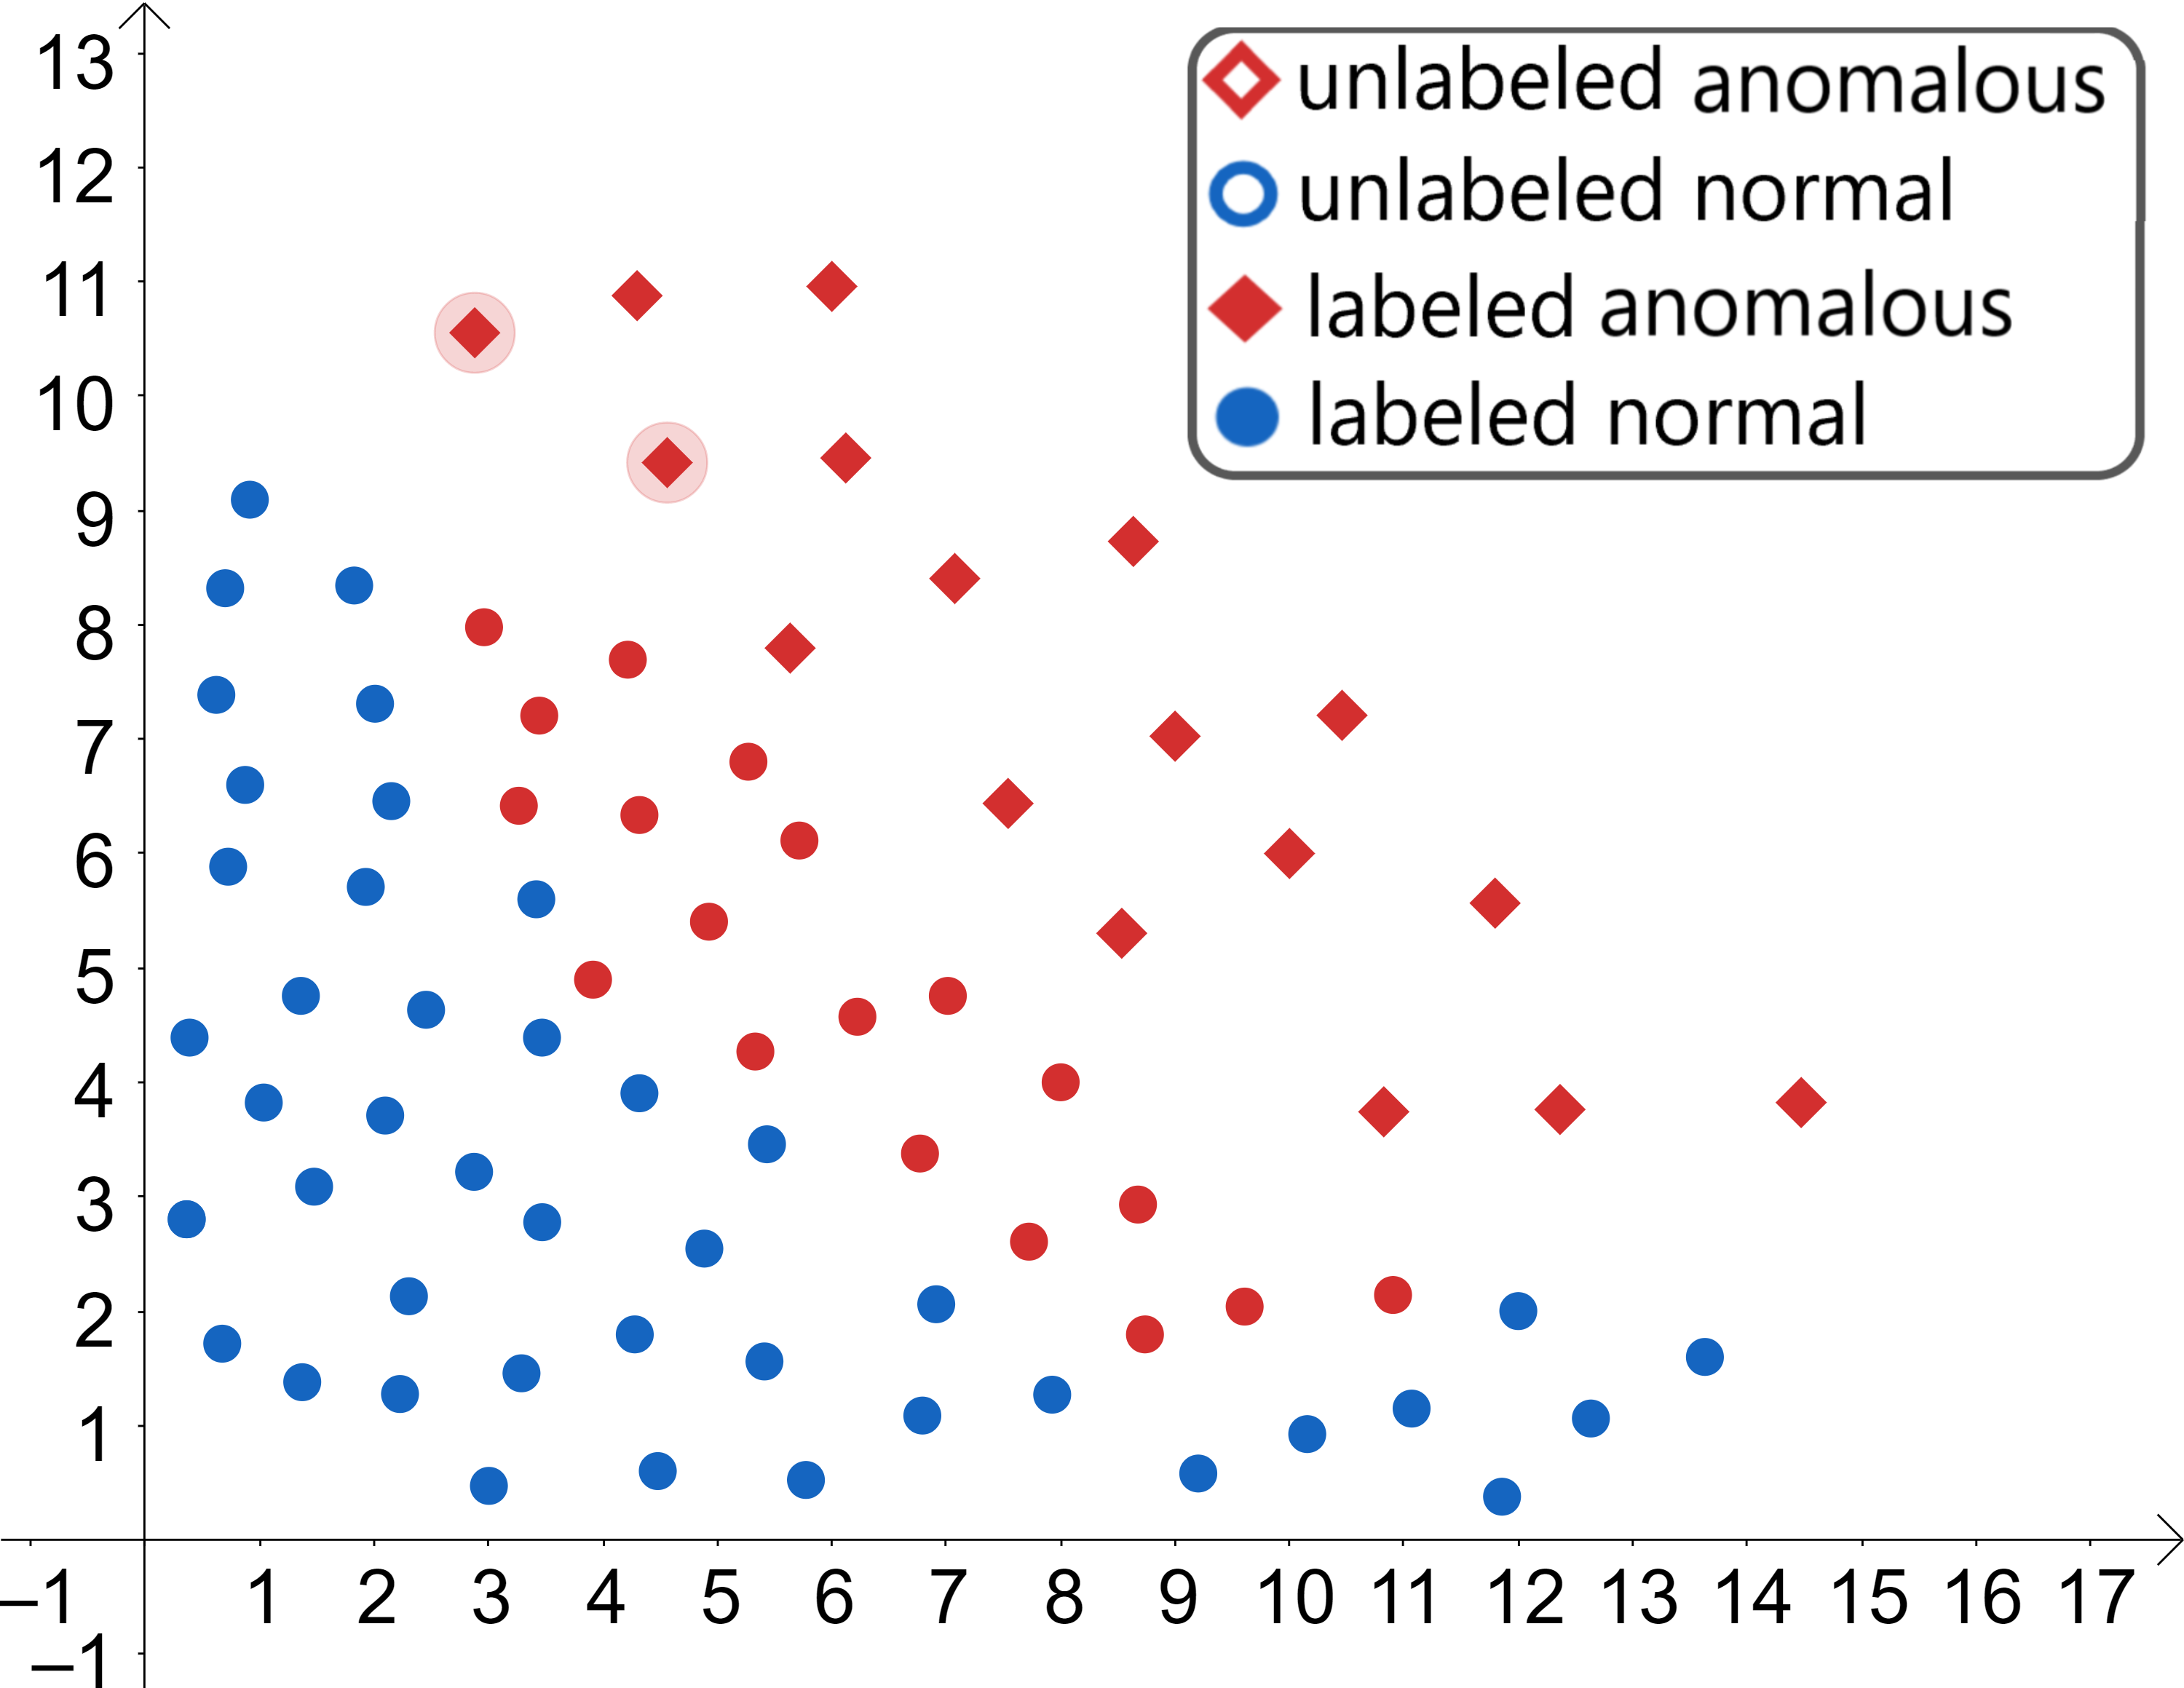
\includegraphics[width=2.6in]{ADS_Journal/PU figures/step4.png}\label{1d}
      \end{minipage}}
	  \caption{The labeling processes of active learning algorithm which labels classification edge samples.}
	  \label{fig:challenges} 
\end{figure*}

\subsection{Definitions}
\label{subsec:kpi}
In this section, we define some key terms of anomaly detection.

\textbf{KPI: }The rapid development of Internet services has brought great convenience to our daily lives. For example, we can use search engines to search online, and we can also use shopping software to buy goods online. In order to ensure the reliability of these Internet services, operators of related companies need to monitor Key Performance Indicators (KPIs) in real time to detect anomalies. A KPI is a time series with the format of (timestamp, value), which can be expressed as $ X = x_1, x_2, \dots, x_n$, where $x_i$ is the KPI value at the time i and n is the length of the KPI  stream~\cite{labelless}.

% KPI streams are roughly divided into two types: service KPI streams and machine KPI streams. Service KPI streams refer to performance indicators that can reflect the scale and quality of web services, such as web page response time, web page visits, and number of connection errors. Machine KPI streams are performance indicators that reflect the state of health of machines (servers, routers, and switches), such as CPU usage, memory usage, disk IO, and network card throughput.


\textbf{KPI Anomaly: }Anomalous data points of a KPI stream means that the data points in the KPI do not meet the expected behavior and are significantly different from the normal data points. For instance, a spike, a level shift, or a dip in a KPI stream likely indicates an anomaly. Typically, an anomalous case always has its context instead of an individual point, which is a collection of continuous points. Figure~\ref{fig:KPI_anomaly} shows three examples of anomalies in KPI streams~\cite{labelless}. 

\textbf{KPI Anomaly Detection: }Anomaly detection for the KPI stream $X$ is to determine whether $x_i$ is an anomalous data point (let $y_i$ = 1 denote an anomalous data point and $y_i$ = 0 denote a normal one). An anomaly detection algorithm typically computes an anomaly score for a data point to indicate the possibility that this data point is anomalous. Operators then set a threshold to determine whether each data point is anomalous or not. Only if the anomaly score at time $i$ exceeds this threshold, $x_i$ will be regarded as an anomalous data point. 

% Through the above definition, we can see that anomaly detection for a KPI stream is  essentially a binary classification problem. In short, anomaly detection is to classify a data point into an anomalous data point or a normal data point. Therefore, the intuitive classification metrics of the two-class classification methods are also suitable for anomaly detection for KPI streams, including precision, recall, and F-score.

% \begin{figure*}
%   \centering
%   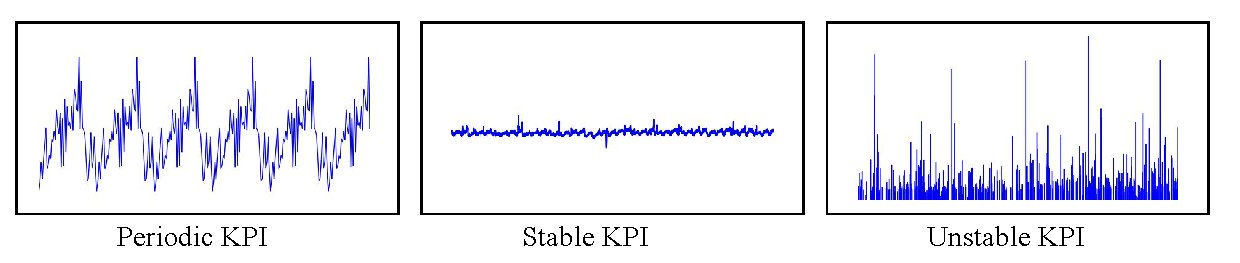
\includegraphics[width=0.9\textwidth]{ADS_Journal/PU figures/different KPI.pdf}\\
%   \caption{The shapes of several KPI streams.}
%   \label{fig:KPI_types}
% %   \vspace{-3 mm}
% \end{figure*}

% \textcolor{red}{
% The difficulties of anomaly detection for KPI streams are:
% \begin{itemize}
%   \item
%   Unbalanced data distribution. In actual scenarios, anomalies are often much fewer than normal data. As a result, there is little anomalous data available for analysis.
%   \item  
%   A large number of KPI streams. Because the actual business system is very complex and will be constantly updated and upgraded, which leads to endless KPI streams.
%   \item 
%   KPI diversity. Figure~\ref{fig:KPI_types} shows the shapes of several KPI streams, we can see some KPI streams are periodic, some are stable, and some are unstable. 
% \end{itemize}
% }

\subsection{Related work of anomaly detection}
\label{subsec:Anomaly Detection Methods for KPI Streams}
Over the years, various algorithms have been applied to KPI anomaly detection, including supervised learning based methods, unsupervised learning based methods and semi-supervised learning based methods.

Supervised learning based methods need to fully label the whole data set. EGADS~\cite{egads} separates forecasting, anomaly detection, and alerting into three separate components and uses AdaBoost [30] to select the most relevant anomalous data points. Opprentice~\cite{liu2015opprentice} ensembles 14 widely-used traditional statistical algorithms with 133 enumerated configurations of hyper-parameters for these algorithms to extract features for the points. Then it trains a classifier using Random Forest. 
Such supervised learning based methods can be well used to learn and detect anomalies if a fully labeled time series is available. However, manual labeling for a large number of emerging KPI streams is not feasible.

Unsupervised learning based methods can not achieve a satisfactory performance. Unsupervised learning algorithms do not require labels of data such as Isolation Forest~\cite{ding2013anomaly} and Donut~\cite{xu2018unsupervised}. Isolation Forest assumes that the anomalous data points are few and different, then constructs tree structure to separate the points from the rest of points until all are isolated. The points closer to the root of the tree will be regarded as anomaly points. Donut is based on VAE, a deep bayesian model performs superior in accuracy. It focuses on normal patterns instead of anomalies and tries to learn the probability distribution of the normal data points. Some other unsupervised based methods, such as Buzz~\cite{chen2019unsupervised} and Bagel~\cite{li2018robust} like Donut are also based on unsupervised learning methods to detect anomalies. However, such algorithms cannot achieve a satisfactory effectiveness. The Internet-based services may suffer from a high false alarms and in turn impact on user experience and revenue.

Semi-supervised learning based methods are halfway between supervised and unsupervised learning. They use unlabeled data to modify either parameters or models obtained from labeled data alone to maximize the learning performance. Malhotra, et al. used stacked LSTM networks for anomaly detection in time series~\cite{Malhotra2015LongST}. They trained a network on non-anomalous data and used it as a predictor over a number of time steps. ADS~\cite{ADSarticle} used clustering and CPLE~\cite{loog2016contrastive} to detect anomaly in time series. Although semi-supervised learning based methods do reduce the cost of manually labeling, it is very difficult for operators to label all the anomalous data points in those specified time series segments and examine the labels back and forth.
% ~\cite{sillito2008semi, ashfaq2017fuzziness, noto2012frac}use semi-supervised learning for anomaly detection in other domains, but are not designed for KPI streams (time series). 
% Although semi-supervised learning based methods do reduce the cost of manually labeling, it is very difficult for operators to label all the anomalous data points in those specified time series segments and examine the labels back and forth.

As discussed above, there are many issues, such as manually labeling all anomalous data (supervised learning based methods), or suffering from a low accuracy (unsupervised learning based methods), or manually labeling all anomalous samples in the selected time series segments (semi-supervised learning based methods).

\subsection{PU learning based methods}
\label{subsec:PU learning based methods}
To address the limitations in Section~\ref{subsec:Anomaly Detection Methods for KPI Streams}, we propose a hybrid solution, which is an important branch of semi-supervised learning to build a binary classifier from only positive (anomalous) and unlabeled samples called PU learning~\cite{PUlearning2017}. While compared with semi-supervised learning algorithms, the initial data labeling required for PU learning is more smaller and the labeling workload is less for the operators.

Traditionally, PU learning is suitable for lots of applications in text detection~\cite{Li2014SpottingFR, Liu2002PartiallySC, putranditional2003, ren-etal-2014-positive} and bioscience~\cite{Mordelet_2011, Yang2014EnsemblePU}. Liu and Lee, et al. firstly regarded the unlabeled samples as negative and utilized the EM algorithm with the naive Bayesian classification method to solve the problem in the text domain. By using the positive documents and the extracted negative documents, it reinitialized the EM algorithm after a few runs and then got the threshold score between positive and negative classes~\cite{putranditional2003}.  Liu, et al. proposed a technique which combines the Rocchio method and the SVM technique for classifier building, while the first step is also treating all unlabeled samples as negative set~\cite{Liu2002PartiallySC}. These methods start by treating all unlabeled instances as negative sets so that it is not applicable for out situation. Because most of the training data in time series anomaly detection is positive. Zhang, et al. improved previous PU learning methods so that it could apply for time series anomaly detection and made it suitable for the unbalanced scenario~\cite{PUlearning2017}. 

In our \name{}, we refer to the PU learning based~\cite{PUlearning2017} to label anomalies as few as possible. We improved the prediction accuracy in anomalous detection of KPI streams by selecting the most reliable anomalous samples in unlabeled data set for labeling and achieve better results than the semi-supervised learning methods.

% Compared with other PU learning based methods, our method  instead of directly treating all as anomalous samples. 

% \begin{itemize}
%   \item
%   Direct use of standard classification methods. A commonly used PU\_learning method is to treat all unlabeled samples as negative samples, and then use labeled data with them to train a standard classifier. The classifier will give each item a score (probability value). Usually the positive samples' score are higher than the negative. So for those unlabeled items, the one with the highest score is most likely to be positive. 
%   \item  
%   PU bagging. A training set is created by randomly combining all positive samples and some unlabeled samples.Use this randomly drawn sample to build a classifier, and treat positive and unlabeled samples as positive and negative samples, respectively.Then apply the classifier to the unlabeled samples that are not in the training set and record their scores.Repeat the above steps, and finally the score of each sample is the average of the scores obtained from multiple iterations.
%   \item 
%   Two-step approaches.Firstly, identify unlabeled samples that can be confidently labeled as negative (called "reliable negatives.") Secondly, train a model with positive samples and unlabeled samples, and then predict the unlabeled samples. Sort unlabeled samples according to the probability, and the previous samples are selected as reliable negatives. Finally, use positive and negative samples to train the standard classifier and apply it to the remaining unlabeled samples. Repeat the above steps to continuously expand the training set and predict the remaining unlabeled samples until the stop condition is met.
% \end{itemize}

% By the observation above, we can see that 


% In order to meet the requirements of anomaly detection of KPI streams, \name{} proposed an improved framework based on PU learning methods. The PU learning in \name{} overview is as follows. (1) Initially, there are only randomly labeled anomalous samples in the existing/historical KPI streams, so the first step is to select credible normal samples from unlabeled data. (2) If there are not enough samples are labeled, we will iteratively label some credible samples. For those that are likely to be anomalous samples, they will be directly labeled as anomalous. For those that are likely to be normal samples, they will be labeled by active learning. (3) Utilize a semi-supervised method to train a final model by labeled and unlabeled data when enough data is labeled.

% In \name{}, active learning is used to label unlabeled samples, thereby helping the PU learning algorithm to obtain more reliable normal samples. ~\cite{Outlieractive}used a selection strategy based on active learning to reduce the classification problem of anomaly detection. ~\cite{Pelleg04activelearning}proposed a novel active learning method to identify rare category records in an unlabelled noisy set with a small budget of data points that they are prepared to categorize. Most of the active learning methods such as~\cite{activelearning2015} selected samples on the classification boundary to label, while via experiments in our KPI streams, choosing the unlabeled data likely to be normal to label is the best selection strategy which is more suitable for KPI streams data.

\subsection{Active Learning}
\label{subsec:Active Learning}
In reality, unlabeled data is quite rich while labeled data is scarce and the cost of manually labeling data is very high. Therefore, we can use a learning algorithm to find the samples useful to us in the unlabeled set, and then present them to domain experts for labeling. After that, we add these labeled data to the training data set. This process is called active learning~\cite{Settles2009ActiveLL}, which has been widely used to label the most informative samples in classification tasks to improve accuracy.

The most important part of active learning is the selection strategy, that is, which data to choose for labeling. For example, the uncertainty criterion measures the confidence of the current model on classifying an instance~\cite{Supportactive2000}, density criterion measures how different an instance is from the labeled data~\cite{Brinker03incorporatingdiversity}, and so on. When training a classifier, the samples at the classification boundary often have high uncertainty. Thus they are usually selected to improve the accuracy of the classifier using uncertainty criterion. While using the various criterion, the samples different from others will be selected.
% For diversity criterion, algorithms hope the information provided by the samples found is comprehensive, and the information provided by each sample is not repeated or redundant. That is, there is a certain difference between the samples.

In \name{}, we use active learning to label unlabeled samples to assist the PU learning algorithm to get more reliable normal samples. Proved by experiments, choosing the unlabeled data likely to be normal to label, rather than labeling data that is on the classification boundary like most active learning methods such as~\cite{activelearning2015}, is more suitable for KPI streams data. Here we simply simulate the labeling process of active learning which labels classification edge samples for theoretical analysis. As shown in Figure~\ref{fig:challenges}, \autoref{1a} illustrates an intermediate state in the process of data labeling. Red represents anomalous samples and blue represents normal samples. At this time, many data points are not labeled. As shown in \autoref{1b}, when using the semi-supervised method to label unlabeled data iteratively, because some normal samples have a high similarity to anomalous samples, it is likely that normal samples are labeled as anomalous samples. When a normal sample is incorrectly judged as an anomalous sample, due to the high similarity between normal samples, more and more normal samples will be added as anomalous samples in the subsequent semi-supervised iteration process as \autoref{1c} shows. The final labeled result is shown in \autoref{1d}. We can conclude that such a selection strategy has the risk of not obtaining 
a good performance of the time series anomaly detection.

\subsection{Clustering of KPI Streams}
\label{subsec:clustering}
Millions of KPI streams are used to monitor Internet-based services in real time to avoid huge losses caused by anomalies. Such a large number of KPI streams is a huge challenge for anomaly detection. As discussed in (Section~\ref{subsec:whether-clustering}), due to the diversity of KPI streams, the results will be inaccurate if only one anomaly detection model is trained for all KPI streams. While, if we train a model separately for each KPI stream, the overhead of anomaly detection is huge. After observation, we found despite the diversity of KPIs, many of them are similar because of their implicit associations and similarities. If we can identify similar KPI streams, and group numbers of KPI streams into a few clusters, we can reduce the overhead in anomaly detection and ensure the accuracy of the results.

According to~\cite{AGHABOZORGI201516}, widely used clustering algorithms can be roughly divided into several groups, including Partitioning, Hierarchical, Grid-based, Model-based and Density-based clustering algorithms. Hierarchical clustering based algorithms require time series to have the same length, and if the length is too long, they are difficult to get a satisfactory result~\cite{CharacteristicBased}. Partitioning clustering algorithms such as K-Means~\cite{MacQueen1967SomeMF} and K-medoids~\cite{kaufman2009finding} need some hyperparameters like the number of clusters $k$, which can not be predetermined definitely in anomaly detection. Grid-based clustering methods are rarely used in time series clustering because they either run very slowly or their results are inaccurate on large data sets~\cite{AGHABOZORGI201516}. Model-based clustering methods assume a model including statistical methods (e.g., COBWEB~\cite{KnowledgeAcquisition}) or neural network methods (e.g., ART~\cite{CARPENTER198754}) for each cluster and find the data that best fits the model. However, these methods often contain strong assumptions (e.g., a Gaussian mixture can model the time series~\cite{865189}) that are difficult to apply on complex data sets. Density-based clustering algorithms are carried out according to the density distribution of samples. The most famous algorithm is DBSCAN algorithm~\cite{ester1996density}.

% Time series clustering is a popular field which has caught a lot of attention in the past 20 years. [20], [21] summarized a large number of methods on this topic, most of which are designed for smooth and idealized data. However, the large number of spikes, dips and level shifts in KPI streams can significantly change the shape of KPI streams. Therefore, the above methods do not perform good for KPI streams.
With reference to the work of Li et al.~\cite{lirobust}, we choose to use the ROCKA (based on DBSCAN) for clustering. It applies moving average to extract baselines which successfully reduce the biases of noises and anomalies. Besides, it uses shape-based distance (SBD)~\cite{paparrizos2015k} as the distance measure, and reduces its algorithm complexity to $O(m log(m))$ using Fast Fourier Transform. Finally, it uses DBSCAN to cluster KPI streams and chooses the centroid for every cluster. 

% Extensive experiments in~\cite{lirobust} have demonstrated ROCKA’s superior performance in clustering KPI streams for large Internet-based services. Please note that applying ROCKA to cluster KPI streams is not our contribution. 



